%\vspace{-.3cm}
\section{Services for sensitive data (TSD)}
\label{sec:tsd}
%\vspace{-.2cm
Project Services Sensitive Data (TSD) 2.0~\cite{tsd} has been created by USIT (The University Centre of Information Technology) at The University of Oslo, to offer a service to researchers in Norway for storing and processing sensitive data, including health data. TSD currently has over 500 projects and over 2500 users, making it the largest sensitive data e-infrastructure in Europe, and is one of the two sensitive data services included in  the service catalog of the European Open Science cloud EOSC-hub~\cite{eosc-hub}.

\subsection{Architecture}
\label{subsec:arch}
TSD is an isolated network infrastructure in which The user area is divided into projects. Each project is isolated from other projects in a separate VLAN, and is accessible only by a set of users who have been registered to this specific project. Project storage is managed by NFS~\cite{nfs}, see~\figref{fig:tsd-arch}. TSD users access and analyse their data through project-space VMs, which are part of a vSphere cluster~\cite{vsphere}. A project-space VM is accessible by all project members, and can be used as a front-end to the system and/or for data processing. A typical project quota includes one Windows Server VM and a collection of Linux VMs. In addition there is a shared project area where software packages and data files (which are NOT classified as sensitive data) are placed. All TSD users have read access to the shared area, while only a few users have write access. Users can log in to their project areas in TSD from the outside world through a two factor authentication system. Three pieces of information must be provided in order to login: username, password, and one-time code (from a Google authenticator which implements TOTP security tokens from RFC 6238).

\begin{figure}[htbp]
	\centering
	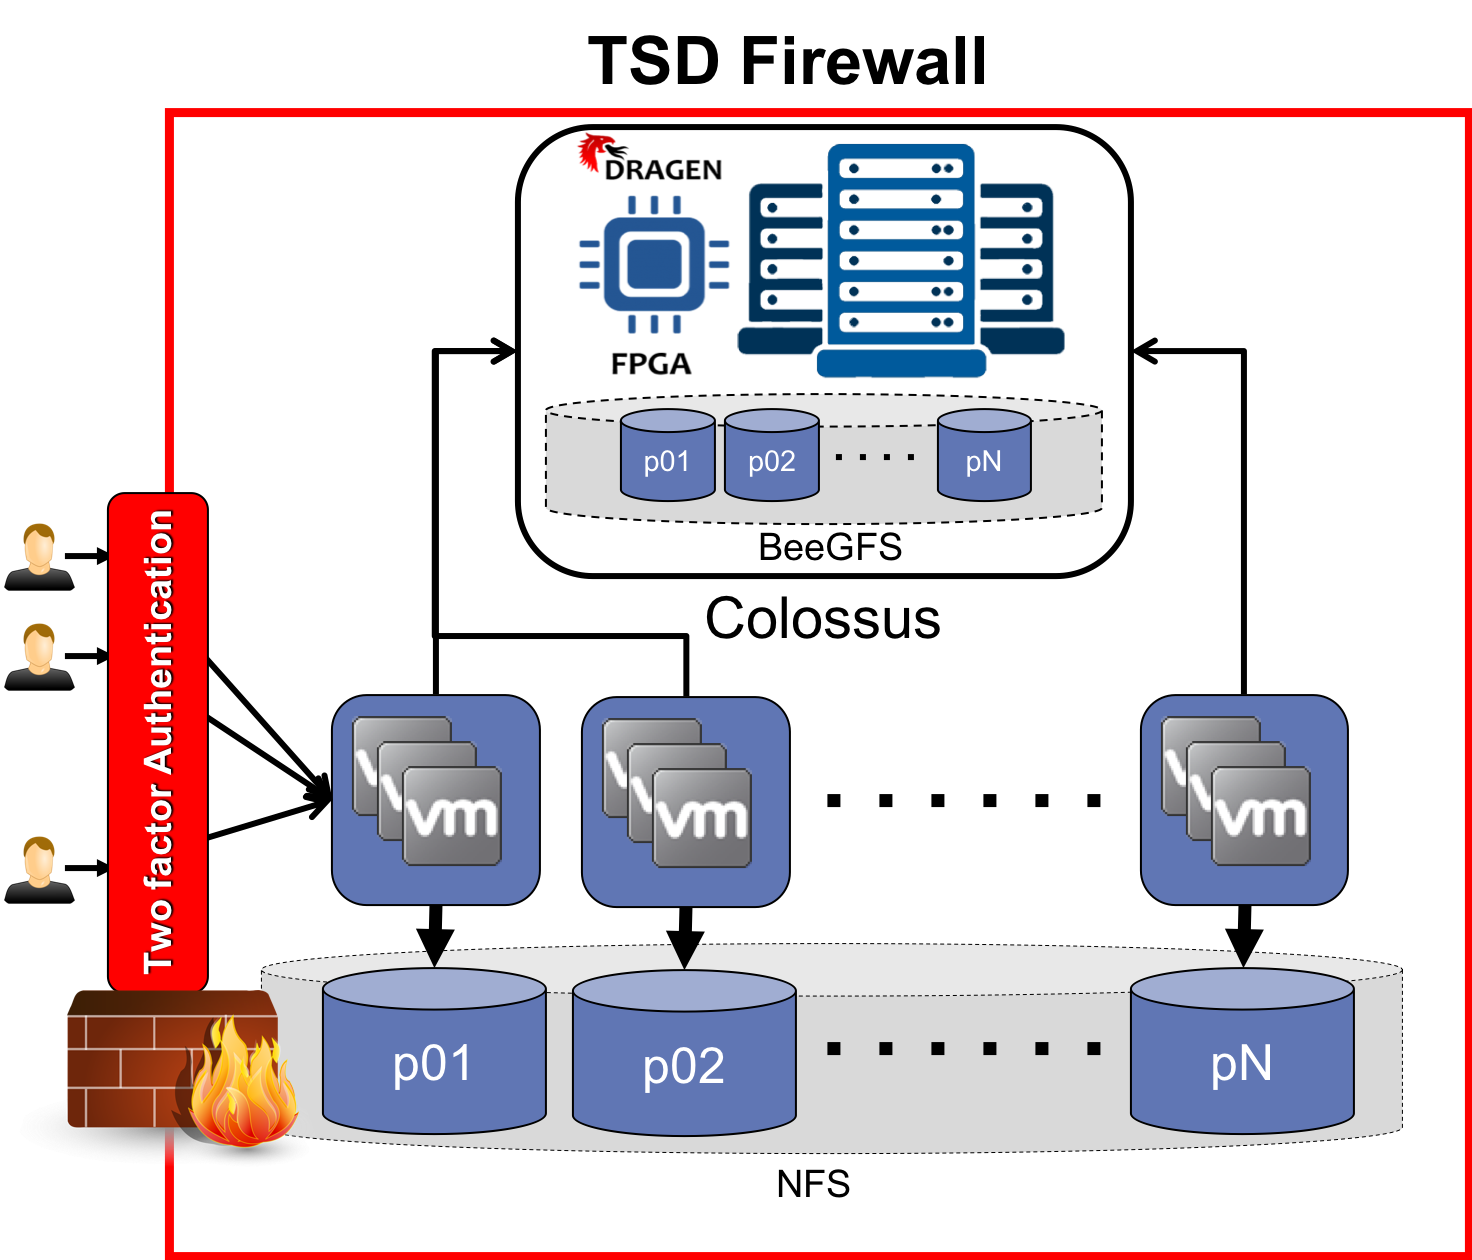
\includegraphics[width=0.5\textwidth]{figures/tsd-arch}                
	\caption{TSD Architecture}
	\label{fig:tsd-arch}
\end{figure}

\subsection{High performance computing}
\label{subsec:tsd-hpc}
High performance data analysis is supported in two options: 

\subsubsection{Colossus~\cite{colossus}}
\label{sec:colossus}
A bare-metal SLURM~\cite{slurm} cluster, that relies on a fast parallel file-system, BeeGFS~\cite{beegfs} which is shared among all TSD projects. A special node of Colossus is Illumina® DRAGEN™ (Dynamic Read Analysis for GENomics)~\cite{dragen} which is a Bio-IT Platform that provides ultra-rapid secondary analysis of next-generation sequencing (NGS) data. The DRAGEN Platform uses highly reconfigurable field-programmable gate array technology (FPGA) to provide hardware-accelerated implementations of genome analysis algorithms, such as BCL conversion, mapping, alignment, sorting, duplicate marking, and haplotype variant calling. DRAGEN platform reduces the run time of variant calling from 30 hours on traditional CPU nodes to 40 minutes. 

\subsubsection{Get Your Own Cluster (GYOC)}
\label{sec:gyoc}
A TSD project PI may request a local virtual HPC cluster which nodes are project-space VM. The queuing system of this virtual cluster can be either SLURM or HTCondor~\cite{condor-paper}. 

\subsection{Data Transfer}
\label{subsec:dataTransfer}

Importing/exporting files into/out-of TSD is done through SFTP connections which are established with the same two factor authentication mechanism, described in \ref{subsec:arch}. The file transfer process, presented in Fig.\ref{fig:file-lock}, takes place in two steps. For importing a file into a TSD project, \lstinline|pXX|, the file is uploaded via SFTP to \lstinline|pXX/import| which is an intermediary area on a NFS file-system that is mounted on an external server, file-lock gateway. Files are then transferred from the intermediary area to a directory in the working project area, \lstinline|pXX/fx/import| through the file-lock service~\cite{file-lock} which is running on an internal VM, file-lock server. TSD also supports a command line REST-API based data import~\cite{tsd-api}. For exporting a file from the project working area to outside the TSD, the user places the file in \lstinline|pXX/fx/export| which is an internal project working area. The file is then transferred through the file-lock service to the intermediary project area \lstinline|pXX/export|, where it can be exported by the user via SFTP. TSD Project administrators have both import and export rights, while regular users have only import but not export rights. 

\begin{figure}[htbp]
	\centering
	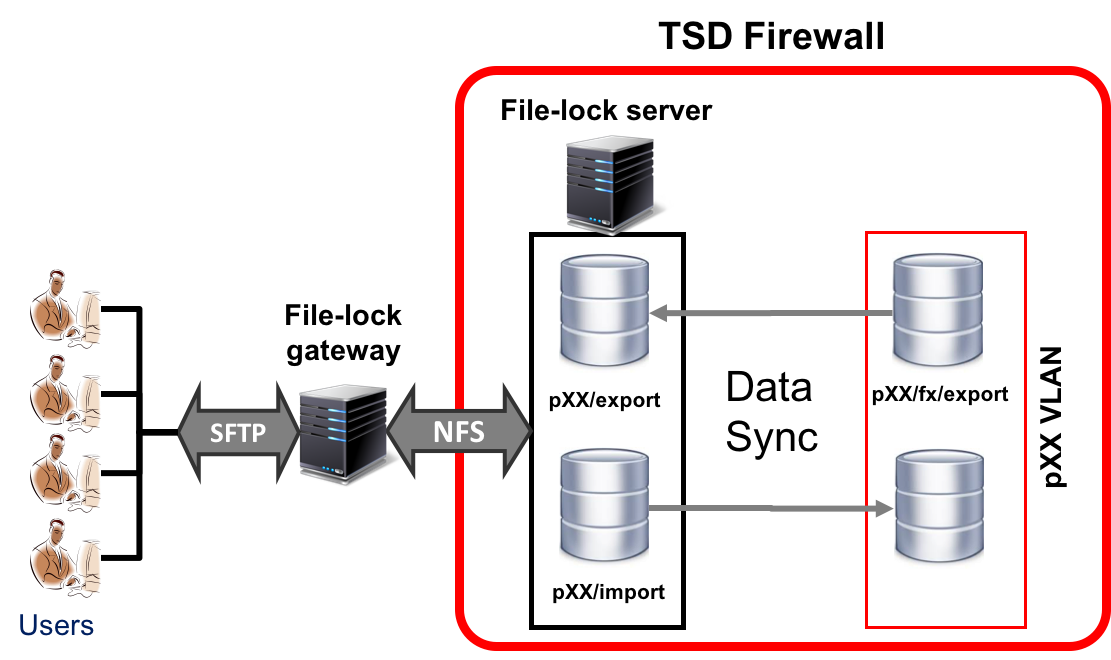
\includegraphics[width=0.5\textwidth]{figures/file-lock}                
	\caption{TSD Data Import/Export}
	\label{fig:file-lock}
\end{figure}
